Data Science is a large domain with many sub-disciplines \cite{sarker2021data, cao2017data}. Thus, the scope needs to be defined and limited for an effective application and evaluation of APE in this field. Additionally, modeling the ontology requires a specific goal and user definition \cite{noy2001ontology} to select an appropriate tool and type set as well as the applied abstraction level. This chapter defines the selected subfields of the data science domain APE is going to be used in, introduces the three use cases for the evaluation, and contains an overview of the ontology, which was created based on these scopes and assumptions.

\section{Limiting the Scope}
In this paper, the data science field is not the target application domain but rather provides a set of methods and tools to transform data and solve problems in other domains. Hence, describing target workflows, which APE will be able to draft, requires defining a subset of data science areas suitable for automated construction and integration into these workflows, as well as the desired user interactions with APE. These areas would contain repetitive and well-defined steps, which could be applied to different problems without requiring structural changes dependent on domain or even problem-specific knowledge. This allows the user of APE to follow the iterative workflow sketching process on the provided semantic abstraction level. Finetuning tool parameters or even implementing structural changes with expert knowledge should still be possible at the end of the construction and exploration process.

\subsection{Targeted Problem Areas}

We select the three areas of \ac{eda}, simple predictive modeling, and text analysis to demonstrate the capabilities of APE when being applied to data science problems.
\begin{enumerate}
    \item \textbf{\ac{eda}} - Exploring given data is usually one of the initial tasks when working with new data \cite{tukey1977exploratory}, and thus, does not yet require problem-specific solutions to get most of the desired results. Steps used during data exploration are, e.g., distribution visualizations, missing value checks, or the application of standard transformations \cite{bruce2020practical}. Nevertheless, some tasks, e.g., mapping keys when merging data from different sources, cleaning data, or deciding on specific ways of handling missing data, might call for knowledge and, thus, tools not contained in the ontology. The extent of necessary changes in the workflow will be evaluated later in this paper.
    \item \textbf{Predictive Modeling} - Besides producing descriptive statistics derived explicitly from the data, predictive analytics applies knowledge gained from historical data to infer new inputs \cite{cao2017data}. Generic tool sequences may deliver a baseline for later models and could be enhanced with implicit insights found in the given data, problem context, and the user’s domain knowledge. Part of the working hypothesis is that the number of needed adaptations in the synthesis output might diminish the benefits of using APE. Hence, the next stage, prescriptive analytics, which may introduce even less reusability between problems, is not in the scope of this paper.
    \item \textbf{Text Analysis} - The third area evaluates working on unstructured data with APE. The additional preprocessing steps to extract tabular data may require new complex data or tool structures and, thus, impact the usability of APE with limited technical expertise and reduce the level of detail in the produced workflows influenceable by the user.
\end{enumerate}
Finally, we define the target audience domains for APE in the data science field. The user is expected to either have some statistical knowledge from related fields, such as cognitive sciences, which would allow them to quickly explore workflows and apply the implementation-independent data science practices to a new problem without having to study a new set of APIs, or to have no statistical knowledge at all, but be able to use their specific domain expertise to provide semantical context to the problem data and explain results produced by the synthesized workflow.

\subsection{User Interactions with APE}

The user interactions with APE can be described in three parts: encoding the available inputs, describing the desired workflow with constraints, and inspecting the synthesized workflow. While the second part may be done entirely in the APE system, input encoding and output inspection or adaptation are heavily influenced by the underlying workflow execution layer. For one, the input data is often tabular, and therefore, any use of column-specific attributes, e.g., data type or column key, requires the input schema to be read and encoded prior to running APE. Furthermore, the workflows may produce multiple statistics, visualizations, and tables, all of which need to be presented to the user in a format that allows them to compare and explore the different workflow variants.

To fulfill these requirements, we decided to parse the APE output graph into a Jupyter Notebook, a standard tool in data science, to interactively write code, display results, and document the process. Kernels exist for more than 50 different languages, such as R, Spark, and Python, and can be used to control the execution of individual steps \cite{kluyver2016jupyter}. The latter was chosen for this project as a backend for its popularity and the vast amount of available libraries. However, the ontology and user interactions remain primarily independent of the specific tool set implementations and could be used with another Jupyter kernel. Documentation of the used tools and types in the notebooks could simplify extending code cells and exchanging steps between notebook variations and APE iterations.

With Python as the backend, the tool implementations will mostly be simplified, wrapped versions of methods from existing data manipulation libraries. The Pandas library \cite{mckinney2011pandas} is commonly used to work with any tabular data and can be used with different input formats. Before calling APE, this library is utilized to extract the attributes required to represent the input objects with APE taxonomy terms. In addition to so-called \texttt{DataFrames}, which contain tables and their metadata, the library also introduces similar \texttt{Series} objects for individual columns and arrays and a collection of commonly used methods to describe and manipulate data. The underlying data in the \texttt{DataFrame} and \texttt{Series} instances is kept in \texttt{ndarrays}, a type from the Numpy library \cite{numpy}. The popularity of the other used libraries, such as Matplotlib \cite{barrett2005matplotlib} and Seaborn \cite{seaborn} for visualizations, scikit-learn \cite{pedregosa2011scikit} for simple modeling, and spaCy \cite{spaCy}, NLTK \cite{loper2002nltk}, and Gensim \cite{vrehuuvrek2011gensim} for natural language processing, will allow for more straightforward adaptations into the APE tool set. Most importantly, the user may use the existing resources associated with these libraries to adapt and finetune the workflows produced by APE.

\section{Defining Evaluation Use Cases}
Three widespread data science problems with openly available datasets were chosen to evaluate APE in the previously defined areas, one for each area. The housing prices dataset \cite{house-prices-Data} evaluates the \ac{eda} workflow with multiple short tool sequences and many user interactions. Next, the Titanic machine learning problem \cite{titanicData} covers the second area. The simple binary classification task predicting survival evaluates the workflow exploration for feature engineering and model selection. Lastly, to test the limits of applying APE’s concept in data science, we chose the IMBD movie review dataset for sentiment analysis \cite{IMBDData}. Due to its unstructured input and binary classification goal, this problem requires different feature extraction steps for the textual data while keeping the modeling simple. Getting an overview of each use case's tool and parameter requirements enables us to model the data flow and create the ontology.

\subsection{Housing Prices}
\ac{eda} is the focus of this evaluation use case. While the other two problems also require understanding the input data, the housing prices dataset has many features with different data types, making it especially interesting for this area. These 81 columns include, e.g., the dependent variable \verb|SalePrice|, the numerical feature \verb|YearBuilt|, and the categorical feature \verb|HouseStyle|. While this regression problem usually requires a model, we will solely focus on the data exploration, which, for this use case, involves tools for data import, descriptive statistics, data cleaning, data transformation, and data visualization. There is no fixed tool order during \ac{eda} since most of the operations are independent of each other. Nevertheless, for this use case, we decided on the step order shown in \autoref{fig:usecase_housing}. Each group contains several activities that will be elaborated on in the next paragraphs. Their order of execution is usually defined in their explanations or displayed in the graph. Optional activities include steps that are typically included in the workflow but technically fall into another area.

\begin{figure}
    \centering
    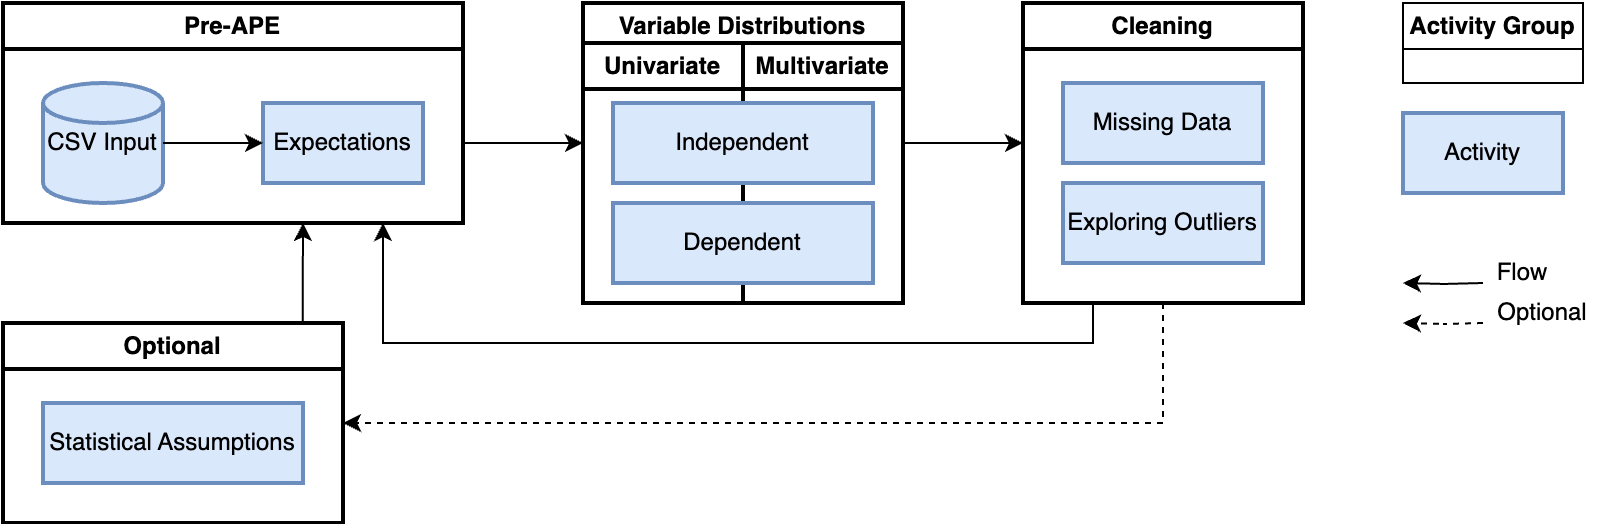
\includegraphics[width=\linewidth]{Tex/images/housing.png}
    \caption{Housing Prices \ac{eda} Steps.}
    \label{fig:usecase_housing}
\end{figure}
\paragraph{Setting Expectations}
Before the APE run, the user should apply his domain knowledge to formulate a set of hypotheses about the dependent variable and the relations of the independent ones. These may be used to modify the input and remove some of the encoded columns to lower the search complexity in APE. Since the data table is a plain CSV file, the pandas loading function can be used and placed in every workflow as the first step. The following tool sequences largely follow the most voted Kaggle notebook for this area \cite{housingprices}.

\paragraph{Exploring Dependent and Independent Variables}
Univariate distributions can be described with descriptive statistics, for instance, value counts for categorical and mean, median, and variance for numerical features. These tools produce a single value for an input column or a series for an entire table. Location and variability should be calculated with skewness and kurtosis or visualized with distribution plots. Similarly crucial for potential models later on is checking multicollinearity, e.g., using correlation matrices. Multivariate relations will be explored using tools like pivot tables, crosstabs, and relationship graphs. Correlation matrices, pivot tables, and crosstabs will change the column or row index and require additional type taxonomy terms to reflect this and keep tool compatibility. The graphs could be customized in size, style, color, etc., requiring specific functions or interchangeable keyword arguments. At this point in the APE workflow, the user may try to explain the produced results in the notebooks using their domain knowledge and adjust the hypotheses accordingly.

\paragraph{Handling Missing Data}
Part of cleaning the given data is deciding how to handle missing data. An important factor is the pattern of the missing values. Determining whether the process is random or biased requires the user to inspect descriptive statistics, filtered table views, and possibly visualized indicator masks. As a result, additional aspects must be reflected in the ontology: Filtering should provide a temporary view of the table, and masks must be the same size as tables to be processed together in operations. Other factors include the number or percentage of missing values in each column, the correlation of these features to the dependent variable, and whether a highly correlated feature with fewer missing values can replace it. If the user decides to drop entries or features, the table index will change, and the resulting memory state in APE needs to encode its incompatibility with the previous version. Alternatively, in some cases, instead of removing table parts, the data can be imputed with simple scalar values, such as mean, median, and mode, or with a model that uses the other feature values to estimate the missing ones. The latter will use the scikit-learn libraries transformers, which have similar technical requirements as the models in the subsequent use case.

\paragraph{Exploring Outliers}
Outliers are another part of cleaning data, and in this use case, they will be handled by inspecting the variable distribution, potentially normalizing it, e.g., centering or scaling, and then deciding whether to remove the entries or not. The process is done for dependent variables before applying the gained knowledge while handling the independent variables. This may be iterated until no outliers are removed. Tools could require threshold values and potential default values for dropping entries, which would also manipulate the table row index. The last areas of data cleaning in this use case that involve changes in the table metadata are handling duplicate values and casting data types. While the first will remove items from the row index, the second will change the table schema.

\paragraph{Test Statistical Assumptions}
Finally, at the end of data exploration, the user might want to test the basic statistical assumptions before training and using a model. We will look at normality, homoscedasticity, linearity, and the absence of correlated errors. The normality of errors in the dependent and independent variables may not necessarily be an issue in large enough data samples. Distribution plots and Box-Cox transformation tests can be used to inspect these before applying appropriate functions if required, such as logarithm, inverse, etc. A new feature might be required to indicate zeros for log transformations. Homoscedasticity, the homogeneity of variance, and linearity can be checked by plotting the features in question, e.g., with scatter plots, and corrected with the previously mentioned transformations and resampling, which would also modify the table index.

\subsection{Titanic}
The Titanic dataset’s task is a binary classification problem in which the target variable indicates whether a passenger survived the infamous accident. The inference can be made based on the 11 other columns in the table, such as \verb|Pclass|, \verb|Sex|, \verb|Age|, or \verb|Fare|. While \ac{eda} is usually part of this modeling use case, the evaluation will focus on preprocessing, feature engineering, model selection, training, and evaluation. Optional steps, which could have technical implications regarding the ontology, are hyperparameter optimization and stacking or ensembling, see \autoref{fig:usecase_titanic}.

\begin{figure}
    \centering
    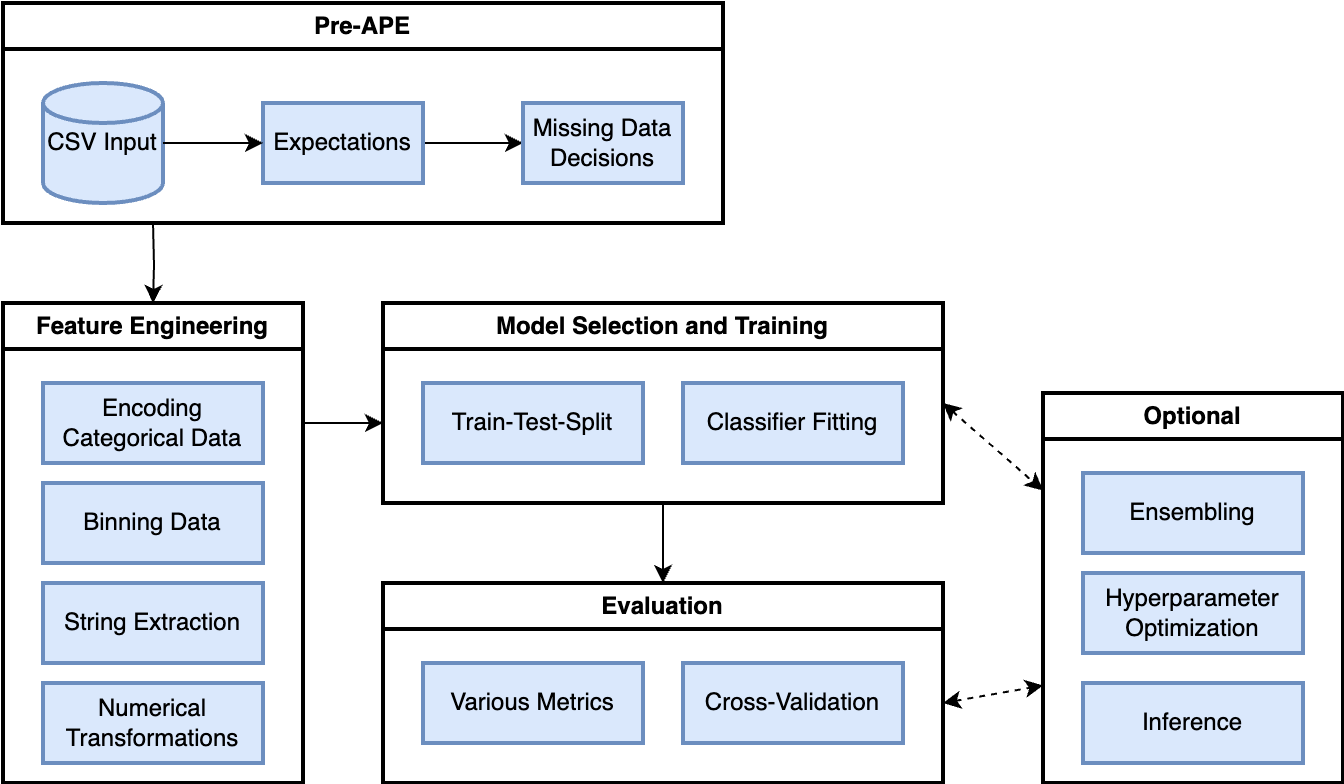
\includegraphics[width=\linewidth]{Tex/images/titanic.png}
    \caption{Titanic Predictive Modeling Steps.}
    \label{fig:usecase_titanic}
\end{figure}

Similarly to the previous use case, the user is expected to have a set of hypotheses about the relationships between the various columns. However, due to the different focus, this time, decisions regarding cleaning data are already made before the first APE iteration. We will again try to recreate the data flow from one of the most-voted Kaggle notebooks \cite{titanic}. The \verb|Ticket|, \verb|Cabin|, and \verb|PassengerID| features will be dropped due to high duplicate or missing value percentages or low correlation to the target variable. Moreover, the \verb|Name| column will be used to evaluate string transformations by applying regular expressions to extract the title. Newly created or transformed features will include a total count of family members on board, a single traveler indicator, and an ordinal age feature. Since the number of columns is relatively low compared to the housing price use case, dropping features before calling APE is less about lowering the complexity for the solver and more about simplifying interpreting the APE outputs.

\paragraph{Feature Engineering}
Creating new columns will modify the table index and could introduce information that is only available at APE or even Python runtime. Further difficulties during feature engineering may occur while encoding categorical or ordinal features. Namely, replacing nominal with numerical values requires extensive domain knowledge and \ac{eda} results, while one-hot encoding them introduces many new unnamed columns. Correspondingly, binning categorical or numerical into new categorical or ordinal features involves a lot of user interactions. It is expected for APE to draft the tool sequence and for the user to test and evaluate parameter combinations.

\paragraph{Model Selection and Training}
The modeling tools will primarily use the scikit-learn classes and functions. Although the titanic problem only requires a classification model, the ontology should also include structures for other types, such as regression or clustering. Model selection relies either on the user's statistical knowledge or on comparing model evaluations against each other and the baseline model, for which we will use the library’s random estimators. Relevant to this problem are supervised learning estimators such as random forests, k-nearest neighbors, or support vector machines, all of which have different parameter sets. As a result, the ontology will model the shared interface only and leave the remaining parameters up to the user. To correctly estimate the risk of models, the dataset needs to be split into training and test or evaluation sets. The associated tool will split the input table into four objects with different indices: feature table and target \texttt{Series} for training and test sets. If \ac{eda} were part of the use case, splitting would occur before the first exploration step to avoid contaminating the modeling process.

\paragraph{Evaluation}
Evaluating the model is done by using a set of appropriate metrics. Since the used models are classifiers, we will use scores such as balanced accuracy, weighted f1, precision, recall, or AUC-ROC. These can be used to estimate the risk of the result of one or multiple train-test splits, e.g., by using cross-validation to achieve a less positive bias. Similar to hyperparameter tuning with grid or random search and ensembling, this requires model and parameter inputs of indefinite length. Grid search would require a set of user-selected parameters to tune and values for each parameter. Correspondingly, ensembling could take an arbitrary amount of models as input to combine them into a new one with voting or stacking. The possibilities of arbitrary user input will be discussed in more detail in the following section and the next chapter. The user may iterate the evaluation process for different models and feature sets by iterating the APE process and adapting the constraints defining the model or by fixing a tool sequence but describing the model with nonterminal taxonomy terms, hence allowing APE to generate the desired workflow variants in one call. The final step inserted by APE could be an inference tool allowing the user to predict new labels with the just-trained model.

\subsection{IMBD Movie Reviews}
The last dataset used to evaluate APE’s capabilities in the data science field is the IMBD movie review dataset for sentiment analysis \cite{imbd,basicnlp}. It is a binary classification problem with labels indicating positive or negative reviews and just one feature: the review text. As previously mentioned, the unstructured nature of natural language texts requires different preprocessing tools, and referencing these and their results requires, in turn, different taxonomy terms. Data import and predictive modeling steps will not differ from the first two use cases. Furthermore, while \ac{eda} will require different tools for natural language texts to, e.g., identify word and sequence lengths, character sets, or unusual vocabulary, user interactions with APE would be nearly identical because of similar tool signatures. Hence, this part of the evaluation will focus on the text feature extraction tools and the user input as shown in \autoref{fig:usecase_imbd}.

\begin{figure}
    \centering
    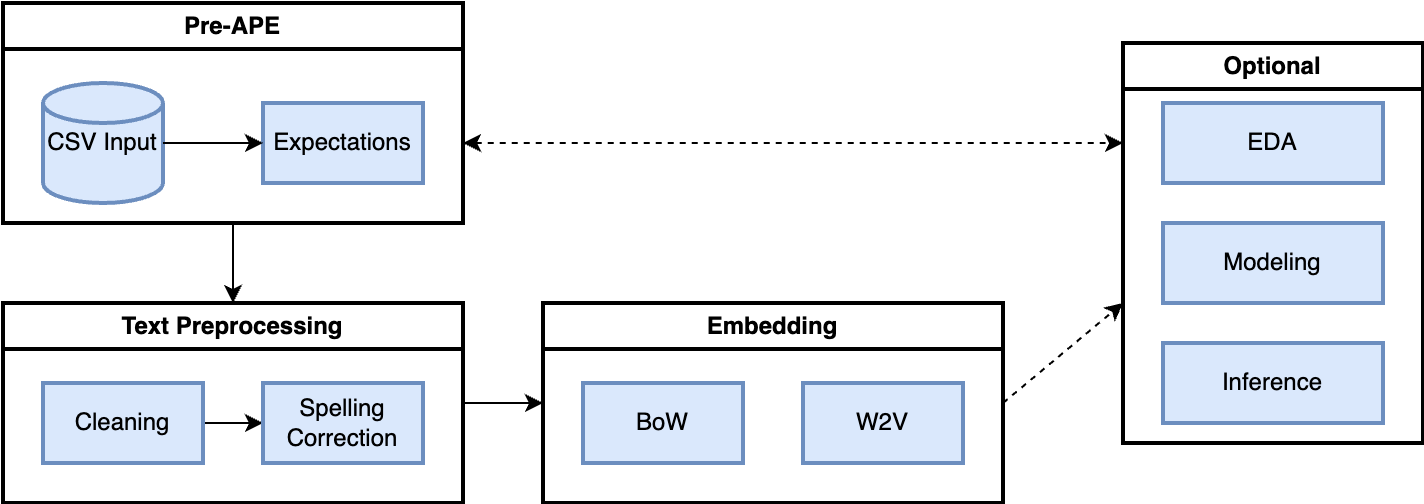
\includegraphics[width=\linewidth]{Tex/images/IMBD.png}
    \caption{IMBD Movie Reviews Text Analysis Steps.}
    \label{fig:usecase_imbd}
\end{figure}

\paragraph{Text Preprocessing}
For this purpose, we will use both simple and semantic-aware string processing tools. HTML tags and other formatting-related markup elements can be removed with the BeautifulSoup library. Unwanted characters or patterns, such as URLs, will be replaced by matching with regular expressions. Finally, we could use dictionaries to replace domain-specific abbreviations. Semantic-aware tools allow us to transform words and sequences based on language-specific attributes. For instance, the spaCy English language models will remove stop words - common words with low semantic importance - and lemmatize the remaining ones, which reduces each word to its base form. Alternatively, the stemmers from the NLTK library could be used to shorten the tokens. Another popular library to transform words is Textblob, which will be used for spelling correction.

\paragraph{Embedding}
Subsequently, the preprocessed reviews must be embedded into numerical vectors before models can be trained. The text feature extractors from the scikit-learn library can create embeddings based on word counts and the given vocabulary, a so-called bag of words. A more complex embedding can be applied with the Word2Vec model from the gensim library, which places each word in a high-dimensional vector space learned from the training data text corpus. Both methods will create large matrices as outputs sharing the same row index as the input table but with a column count dependent on the review texts’ content. The latter is unavailable at the APE runtime and should thus not be regarded while modeling the ontology. However, the extent to which the user can still interact with these produced types without requiring substantial changes in APE compared to the other two use cases will be a prominent topic during the evaluation.

\section{Modeling the Ontology}
By defining the problem, identifying use cases, and extracting requirements, we implicitly answered vital questions whose answers will steer the ontology modeling process \cite{noy2001ontology}. Namely, we specified the purpose to be a semi-automated search, where the user would iterate the synthesis process and adjust the configuration and constraints. Furthermore, we expect the resulting workflow to be executable but not necessarily optimal. Additional crucial aspects discussed in this section are the level of detail in the taxonomies and the differentiation of tool inputs vs. parameters, which we have already touched upon during the use case introductions. Heuristics are currently not natively supported by APE and, therefore, not mentioned here. However, we will introduce them into the ontology when changing the backend of APE in \autoref{sec:asp_backend}. Finally, the collaboration and social contract aspects of this new domain ontology are not covered here as we mostly inherit the advantages of the APE ontology format. The only difference is that the taxonomy structures are primarily adopted from the used tool libraries' class hierarchies, which may simplify working with the ontology for those already familiar with these standard data science tools. The following subsections will provide an overview of the tool taxonomy, the type taxonomy with its dimensions, and their interactions in the tool annotations.

\subsection{Tools Taxonomy}
The tools needed to synthesize workflows described in the three use cases can be separated into the six overlapping sub-taxonomies \verb|EDAFeatureEngineering|, \verb|Plotting|, \verb|Modeling|, \verb|Encoding|, \verb|Embedding|, and \verb|Utility|. In contrast to the type sub-taxonomies, the tool hierarchies are primarily based on their semantic effect instead of their associated libraries, especially since many of the used libraries share functionalities. For instance, the scikit-learn library provides a tool to plot their decision tree objects as a graph. While most of the 113 leaves in the tool taxonomy are implemented as wrappers for common library function call sequences, some are required to ensure compatibility with APE, namely, those in the Utility sub-tree.

\begin{figure}
    \centering
    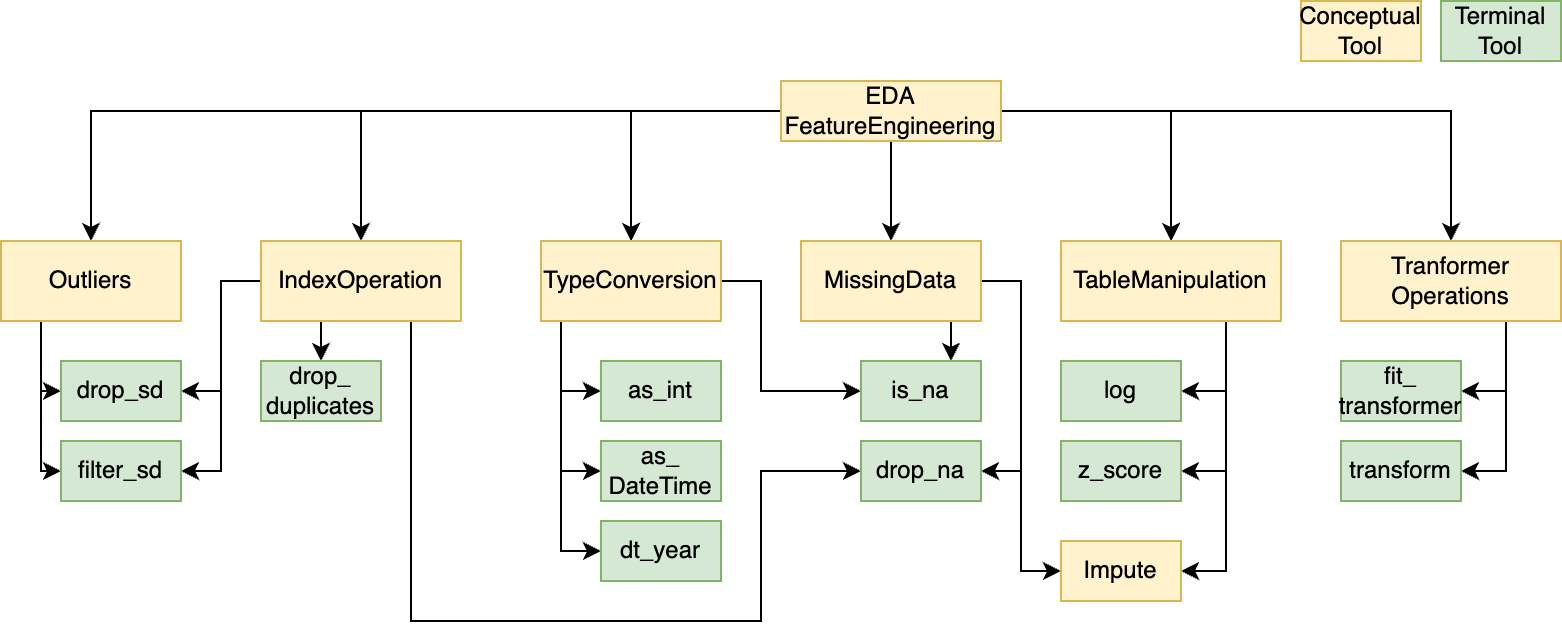
\includegraphics[width=\linewidth]{Tex/images/ToolsSimple.png}
    \caption{Selection of Tools from a Simplified \ac{eda} and Feature Engineering Sub-Taxonomy.}
    \label{fig:subtax_eda}
\end{figure}

The first sub-taxonomy for \ac{eda} and simple feature engineering primarily contains methods from the Pandas library. A representative selection of tools can be seen in \autoref{fig:subtax_eda}. The implementations of this sub-taxonomy allow for table and column description, handling missing values, string manipulation, pattern extraction, table reshaping, and column transformation. Even though the transformer objects are part of the scikit-learn library and share similarities in their interface with the models, they are categorized into this sub-taxonomy as these classes are intended to modify tabular data. The figure shows how, in addition to being organized by their purpose, e.g., table summary statistics or string operations, the tools are also agglomerated by their operation type, such as whether they manipulate an entire table or just one column, whether the row index is getting modified, and if the operation is in-place. Consequently, each tool may be a child node of multiple parent nodes, all of which can be used by the user to describe the desired tool. For instance, a tool state node constrained by \verb|TypeConversion| and \verb|MissingData| could be instantiated by the leaves \verb|isna| or \verb|notna| in APE.

Next, the Plotting sub-taxonomy comprises tools for data visualization functions from the Seaborn, scikit-learn, and Wordcloud libraries. They cover tasks like graphing variable distributions, relationships, and trends, as well as more complex graphs, like tree feature importance plots and word clouds. Additional boilerplate function calls were added to the implementations to enable figure customization, such as setting graph size or rotating labels. These aspects can be controlled with optional keyword arguments through different tool modes in APE or by the user while fine-tuning the workflow. Together with the previous sub-taxonomy, these tools fulfill the majority of the housing price use case requirements.

While the scikit-learn library is also used for data transformation, its primary purpose in this ontology is the enablement of classification workflows as outlined by the Titanic problem. Indeed, all model classes stem from scikit-learn, as do the helper functions for the other workflow steps: model selection and evaluation. However, due to the SAT problem encoding in APE, accessing features and target labels separately, as required by these models, proves difficult. This issue of handling tables, a dominant type in data science, is one of the main challenges in this paper and will be discussed in detail in the following sections and chapters. Here, utility functions are added to control the flow of tabular data in APE in the training and prediction steps.

Similar issues attributed to the tabular structure occur when encoding nominal or ordinal features. Both steps are essential since the used model classes require all inputs to be numerical and are implemented by extended Pandas functions. Furthermore, the text analysis use case introduces the need for text embeddings, vectorized representations of unstructured data that models can handle. Like the encoding tools, vectorization will modify the table column index, and the resulting shape is unknown at APE runtime. Moreover, in most cases, the embedding table has such a high column count that dimensionality-reduction tools are deployed to lower the complexity before further analysis. They are another set of tools that will modify the table index and are implemented by scikit-learn transformers in this ontology.

\subsection{Type Taxonomy}
To properly represent the different data types in our use cases, we utilize APE’s capability to handle multiple dimensions in the type taxonomy. In addition to the primary dimension \verb|DataClass|, the smaller sub-taxonomies \verb|DataState|, \verb|Statistical| \verb|Relevance|, and \verb|DataSetIndex| describe each type state in the workflow synthesis. The advantages and disadvantages of adding these optional dimensions will be analyzed in the evaluation \autoref{ch:evaluation}.

\subsubsection{Primary Dimension - Data Class}
\begin{figure}[h]
    \centering
    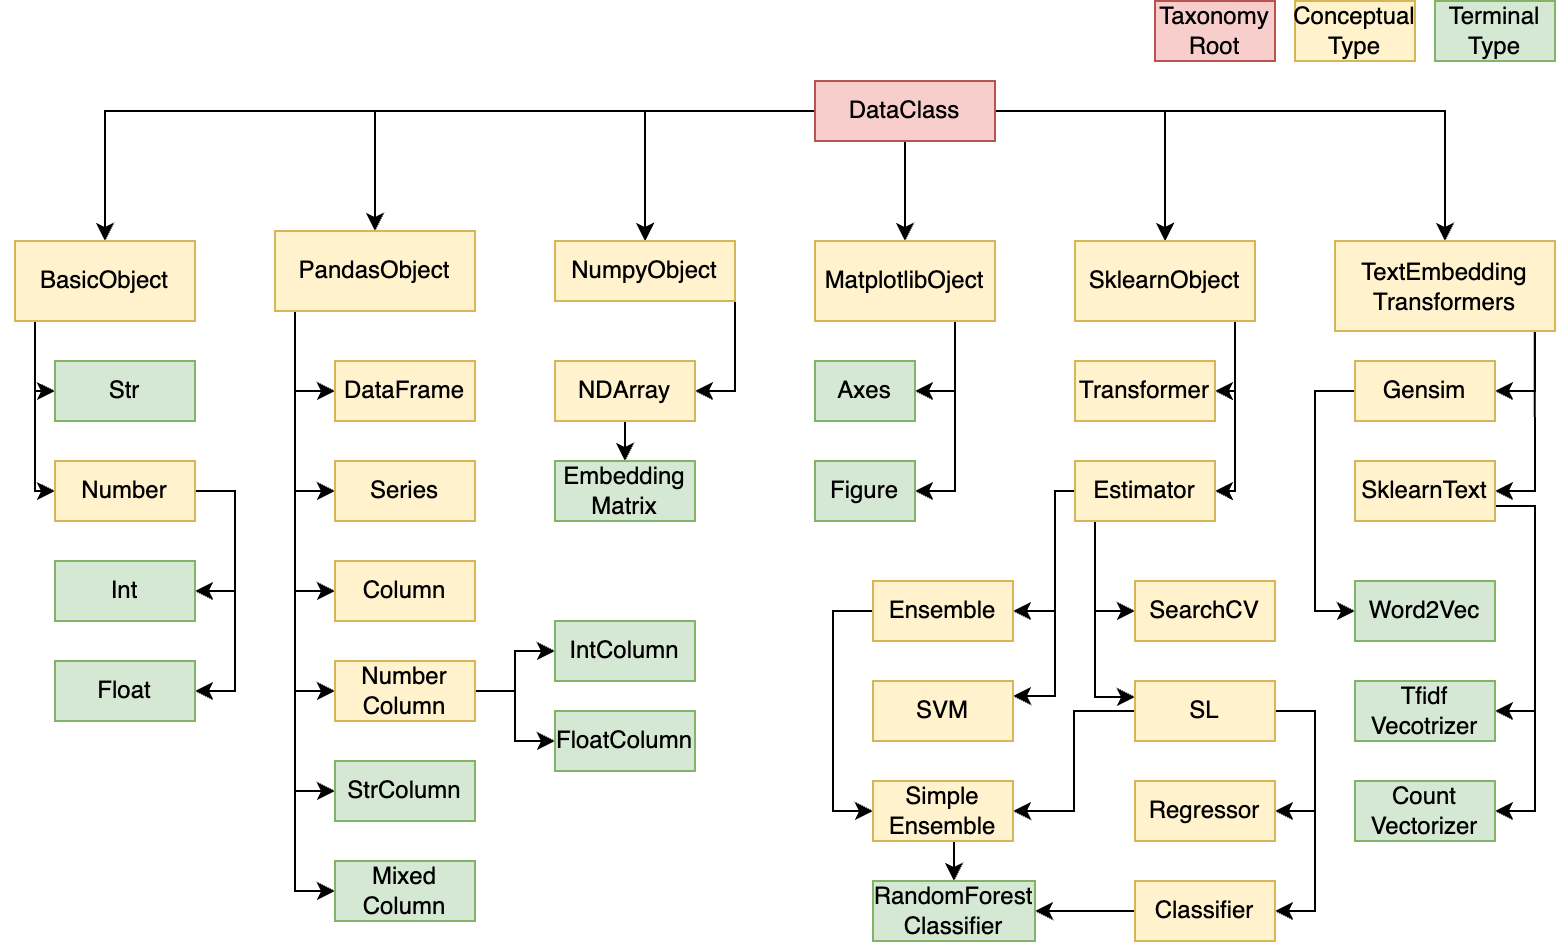
\includegraphics[width=\linewidth]{Tex//images/DataClassSimple.png}
    \caption{Selection of Types from the \texttt{DataClass} Dimension.}
    \label{fig:subtax_dataclass}
\end{figure}
As visualized in \autoref{fig:subtax_dataclass}, the types in the primary dimension are categorized into six disjunct sub-taxonomies: \texttt{BasicObject}, \texttt{PandasObject}, \texttt{MatplotlibObject}, \texttt{NumpyObject}, \texttt{SklearnObject}, and \texttt{TextEmbeddingTransformers}. While the first five hold types from their respective libraries, the last sub-taxonomy consists of various text-processing transformers. Here, multiple inheritances were only required for the scikit-learn objects, which are grouped by model and target label type, e.g., \verb|DecisionTreeClassifier| being both \verb|SL| - supervised - and \verb|Tree| - a tree model.

Basic types can either be outputs of descriptive statistic functions or user-defined custom inputs passed in the configuration or constraint file. While their value does not influence the workflow synthesis process, they are later required for notebook construction. For this reason, we are using APE’s implicit dimension \verb|APElabel|, which is created at runtime from all the \verb|APElabel| values in the input type nodes. For instance, if an input of type \verb|Int| had the label \verb|42|, that value may get passed along to a tool accepting a parameter of type \verb|Int|. The limits of this method will be discussed in the following subsection and chapter.

Additional potential problem sources are the complex types, especially the tables implemented here as Pandas \texttt{DataFrames}. These tables consist of multiple columns, all of which may hold different basic types. Some tools require the entire input table to have a specific type. In contrast, others produce tables with a particular format or type, such as correlation matrices, which always contain numbers, or classification reports, which have a fixed column index. In response to these inherent requirements, we use detailed \texttt{DataFrame} object types and add two more \texttt{PandasObject} subtypes: \texttt{Column} and \texttt{Series}. To address columns individually, each column in a table is encoded into a type node as follows: A table with a column containing strings would be encoded into the detailed table type node and a \texttt{StringColumn} node. If a column is separated from a table and write operations do not modify the source table anymore, its \texttt{DataClass} type changes to \texttt{Series}, e.g., when the input table is split into a feature \texttt{DataFrame} and a target label \texttt{Series}. At the Python layer, values in these Pandas objects are stored in Numpy arrays. However, to avoid the decrease in technical abstraction, the only Numpy type used in the three use cases is \texttt{EmbeddingMatrix}, which is required for text feature extraction.

The visualizations produced by the previously mentioned libraries are stored in Matplotlib objects, namely \texttt{Figures} and \texttt{Axes}. Each \texttt{Axes} object can hold a plot with its metadata and can be used to set, e.g., label orientation or scale. \texttt{Figures}, in turn, contain one or more \texttt{Axes} objects and control aspects such as layout and overall size. As a tuple, they are the standard output signature for most of this ontology’s plotting tools.

Finally, the \verb|SklearnObject| and \verb|TextEmbeddingTransformers| sub-taxonomies include complex feature engineering and modeling classes. Namely, instances from these collections differ in their requirement to be trained or fitted before any data transformation or prediction is possible; see \autoref{par:data_state}. The data class \verb|Sklearn| \verb|Object| comprises dummy estimators and various classification, regression, and clustering models. Including different architectures and baseline models enables assessing the exploration potential of APE in a modeling workflow. On the other hand, \verb|TextEmbeddingTransformers| has only three concrete transformers due to the text analysis use case focusing on the feasibility of interactions with the produced output structures instead of workflow exploration or exploitation.

\subsubsection{Secondary Type Dimensions}
Each secondary dimension adds information already available in the input data or inferable by APE during the synthesis to increase the probability that the resulting workflow is syntactically and semantically correct. However, applying this level of detail is optional, and the user may always utilize default values, such as the root type \verb|DataState| for any data state, including none, or \verb|NoState| for explicitly none, as seen in \autoref{fig:subtax_datastate}.

\begin{figure}[h]
    \centering
    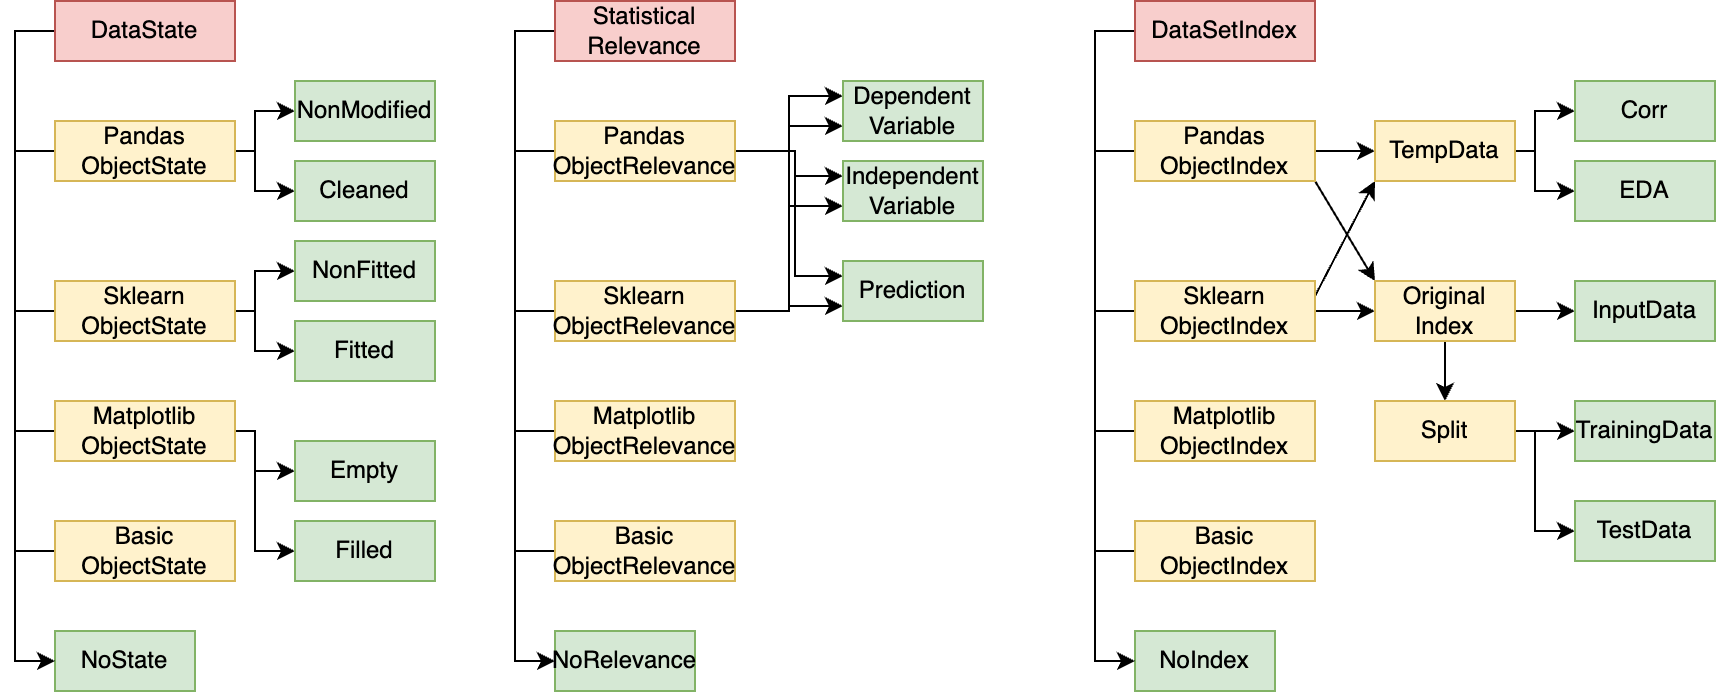
\includegraphics[width=\linewidth]{Tex/images/OtherDimsSimple.png}
    \caption{Secondary Dimensions with fallback types.}
    \label{fig:subtax_datastate}
\end{figure}
\paragraph{Data State}\label{par:data_state}
This dimension is required for scikit-learn objects. Namely, it acts as a flag differentiating fitted and non-fitted models and transformers. Since some tools are only available for one of these states, adding this information avoids non-executable scikit-learn function calls. Furthermore, the data state dimension allows users to wield more fine-grained control over Pandas and Matplotlib objects. If feature engineering is part of the workflow, one requirement may be to normalize numbers and clean textual data, and \texttt{Figures} may only be accepted as output if they are filled with a plot. Type nodes of other data classes have no dedicated data state values and, thus, use the \verb|NoState| type.

\paragraph{Statistical Relevance}
The next dimension is optional for syntactical correctness. However, adding its types to the ontology provides more detail to the tool annotations and, as a result, reduces the number of required user constraints to reach the desired workflow. Statistical relevance primarily applies to Pandas objects and describes their role in a modeling workflow. Moreover, these types can also be applied to objects from the scikit-learn library to specify their purpose. For instance, a transformer or estimator may have been fitted to impute or predict dependent or independent variables. Other data classes do not have specific types in this dimension and share the \verb|NoState| type.

\paragraph{Dataset Index}
Finally, the dataset index dimension assists in making sure that steps using tools accepting two or more tables share the same table index and, hence, are executable. In a modeling workflow, a feature \texttt{DataFrame} may be transformed and cleaned. However, if some index modifying operation, such as dropping duplicates, was applied, the resulting \texttt{DataFrame} is no longer compatible with the original target label \texttt{Series}, and the notebook, while syntactically correct, would raise an error at runtime. The available index types are split into original indices, derived directly from the input data or during the modeling workflow, and temporary indices, created during data exploration for a specific purpose, such as a correlation matrix. In addition to being available to Pandas objects, these types can be applied to Matplotlib and scikit-learn objects to document their data source. The \verb|NoState| type is assigned to objects of the remaining data classes.

\subsection{Tool Annotations}
Modeling the ontology is an iterative process, and each time a new set of tools or types is added, the tool annotations, which combine these taxonomies, are potentially subject to modification. These derived transition rule changes efficiently reveal conceptual flaws in the ontology, as we will show in \autoref{sec:native_ape_challenges}. The tool signatures closely resemble those of standard data science libraries, with the table access concept as the central assumption and starting point for tool modeling. Since the Pandas library has an integer position and label-based row and column indexing system\cite{mckinney2011pandas}, any tool in the ontology that accesses a specific part of a \texttt{DataFrame} also requires the index parameter. However, creating entries for each row or integer position in a dataset is impractical. For this reason, APE-synthesized table access relies on column labels. For instance, this simplified signature for a scatterplot \verb|(DataFrame, NumberColumn, NumberColumn) -> (Figure, Axes)| illustrates how APE represents the parameters for the source table and the x and y value columns.

Currently, most leaves in the tool taxonomy are overloaded in their implementation. These differ in their optional parameters, such as graph coloring or styling, but also regarding parameter types, as exemplified by the scatterplot function. In addition to two columns for x and y values, it accepts column label parameters for marker hue and style, as follows:
\begin{verbatim}
(DataFrame,NumberColumn,NumberColumn,Column) -> (Figure,Axes)
(DataFrame,NumberColumn,NumberColumn,Column,Column) -> (Figure,Axes)
\end{verbatim}
APE unifies these rules during the workflow search, and each term is assigned a terminal type according to the taxonomies. Consequently, the type states corresponding to the first three parameters in the scatterplot signature could be unified with their terminal \verb|DataClass| sub-types, such as
\begin{verbatim}
(MixedDataFrame, IntColumn, FloatColumn)
\end{verbatim}
However, the SAT solver still requires explicit state transitions despite APE allowing implicit type and tool states in its input files. As a result, any implied relation between a tool's input and output parameters must be made explicit. If, e.g., a tool changes the \verb|DataState| of a \verb|SklearnObject|, a non-terminal \verb|DataClass| type, from \verb|NonFitted| to \verb|Fitted| the implied unifications should have the following form: \begin{verbatim}
((X, NonFitted), …) → ((X, Fitted), …)
    where X is terminal sub-type of SklearnObject
\end{verbatim}
A preprocessing step is introduced to circumvent this lack of generic type variables in APE tool signatures, transforming these implied input-output transitions into explicit terminal rules. Notably, for this ontology, the instantiation step following generation and constraint patterns, not unlike a declarative solver, produces approximately 1000 tool modes from around 100 tools.

\section{Discussion}
This chapter defined the targeted problem areas and users for this ontology. Next, three use cases were selected to evaluate \ac{eda}, predictive modeling, and text analysis. Based on the derived requirements, we modeled the ontology consisting of tool and type taxonomies and tool annotations. However, the obtained result is a mere starting point representing everyday data science tools and types. It is meant to be extended for additional use cases and adapted to fit technical requirements.

At the current stage, the ontologies functionality is still theoretical when combined with APE. Potential challenges include the complexity of the created SAT problems and the usefulness of the various APE outputs. The latter is because many overloaded tools could lead to all found workflow variants being structurally identical with slight parameter changes. Furthermore, the scalability of this ontology is questionable: On one hand, the taxonomies roughly imitate the class hierarchy of each used library and should be navigable with data science knowledge. On the other hand, the applied technical abstractions do not follow an existing common standard. Thus, it might be challenging for various parties to maintain these novel taxonomies with their multiple inheritances.

The following two chapters will introduce two approaches to using these ontologies. They will address existing and new challenges arising from each course and apply the required modifications to the ontology. However, other aspects, such as maintainability, will not be evaluated and are subject to future work.